\chapter{Fundamentação Teórica}

  Nesse capítulo será feita a fundamentação dos principais assuntos presente nesse trabalho: a heurística construtiva, a heurística de refinamento, as metaheurísticas e a programação linear. Nas seções seguintes serão descritas os aspectos teóricos e os principais métodos relacionados a esse trabalho.

	\section{Heurísticas Construtivas}
		As técnicas de resolução heurísticas se utilizam de processos intuitivos afim de obter uma boa solução, a um custo computacional aceitável, ou seja não garante a otimalidade de um problema. O objetivo é obter em um tempo reduzido uma solução tão próxima quanto possível do ótimo global. 
		
		Uma heurística é dita construtiva quando a construção da solução se dá elemento por elemento. A forma de escolha dos elementos variam de acordo com a estratégia e a função de avaliação adotada, essa escolha deve levar em consideração o benefício da inserção de cada elemento para a solução final, escolhendo sempre o \emph{melhor} elemento em cada passo.
		A Figura \ref{heuristicaconstrutiva} mostra o pseudocódigo para a construção de uma solução inicial para um problema de otimização que utiliza uma função gulosa \emph{g(.)}. Nesta figura, \emph{$t_{melhor}$} indica o membro do conjunto de elementos candidatos com o valor mais favorável da função de avaliação \emph{g}, isto é, aquele que possui o menor valor de \emph{g} no caso de o problema ser de minimização ou o maior valor de \emph{g} no caso de o problema ser de maximização.
		
\begin{figure}[ht]
	\centering
	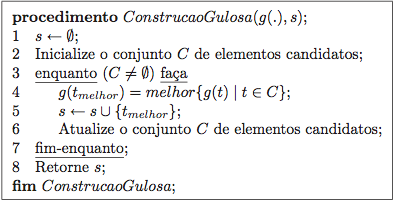
\includegraphics[scale=0.7]{./img/heuristicaconstrutiva}
	\caption{Heurística de construção gulosa de uma solução inicial}
	\label{heuristicaconstrutiva}
\end{figure}

Uma outra forma de obter uma solução inicial é escolhendo os elementos candidatos aleatoriamente. Isto é, a cada passo, o elemento a ser inserido na solução é aleatoriamente selecionado dentre o conjunto de elementos candidatos ainda não selecionados. A grande vantagem desta metodologia reside na simplicidade de implementação. Segundo testes empíricos , a desvantagem é baixa qualidade em média da solução final. Essa técnica é recomendada quando a característica do problema torna mais fácil o refinamento do que a construção de uma solução \citep{notasmarcone}. 

A Figura \ref{construcaoaleatoria} mostra o pseudocódigo para a construção de uma solução inicial aleatória para um problema de otimização.

\begin{figure}[ht]
	\centering
	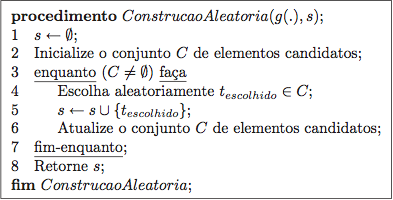
\includegraphics[scale=0.7]{./img/construcaoaleatoria}
	\caption{Heurística de construção aleatória de uma solução inicial}
	\label{construcaoaleatoria}
\end{figure}

Para melhores resultados essa etapa deve ser seguida de um refinamento.

\section{Metaheurística}

A utilização de métodos exatos para a resolução de problemas reais envolvendo otimização combinatória é restrito. Isso acontece pois com o aumento das instâncias envolvidas, o número de soluções possíveis cresce exponencialmente, fazendo com que as operações necessárias para a sua resolução não possa feita em tempo viável com os computadores atuais.  

Para contornar essa limitação e obter soluções para esses tipos de problemas, os pesquisadores desenvolveram técnicas que são capazes de guiar o procedimento de busca e assim encontrar "boas" soluções \cite{maritan2009}. Esses algoritmos, denominados heurísticas \cite{dias2006}, encontram essas soluções utilizando pouco recursos computacionais, porém não garantem a solução ótima do problema. Na prática, geralmente, uma boa solução é suficiente, já que a tomada de decisão tem que acontecer em um curto espaço de tempo.

As heurísticas apresentavam a restrição de ser aplicáveis a uma classe restrita de problemas. Para contornar esse problema, foram desenvolvidas técnicas mais generalistas que foram denominadas de metaheurísticas. As metaheurísticas podem ser definidas como sendo um método heurístico para resolver de forma genérica problemas de otimização com a capacidade de escapar de ótimos locais. heurísticas de caráter geral e com capacidade de escapar de mínimos locais. A idéia utilizada, normalmente, é obtida de algum evento natural como sistemas biológicos, da física ou da inteligência artificial.

As metaheurísticas podem explorar o espaço de soluções basicamente de duas formas: as metaheurísticas de busca local e as metaheurísticas de busca populacional. Nas metaheurísticas de busca local, o procedimento de busca utiliza uma solução como ponto de partida em cada iteração. As metaheurísticas GRASP, Simulated Annealing eBusca Tabu podem ser citadas como exemplos de metaheurísticas ponto-a-ponto. Nas metaheurísticas de busca populacionais, soluções de boa qualidade são combinado com o intuito de produzir soluções melhores. Podemos citar como exemplo de métodos populacionais, os Algoritmos Genéticos, Colônia de Formigas (Ant Colony System), Particle Swarm Optimization (PSO) etc \cite{maritan2009}.

Nas próximas seções serão apresentados a metaheurística GRASP e o método de busca local ILS.

\subsection{Greedy Randomized Adaptative Search Procedure (GRASP)}

Essa seção descreve a metaheurística GRASP, que foi  desenvolvida por Feo e Rezende \cite{resende1995}, e cujos conceitos serão utilizados na metodologia proposta para resolução do PCTA.
A metaheurística GRASP é um método iterativo do tipo \textit{multi-start} formado por duas fases: uma fase de construção de uma solução e outra de busca local. A fase de construção objetiva gerar uma solução viável para o problema proposto. E a de busca local, através de estrutura de vizinhanças, tenta melhorar essa solução. 

O pseudocódigo do GRASP é apresentado no algoritmo \ref{alg:grasp}. Na linha 1 o custo da função objetivo da melhor solução encontrada é inicializada com $\infty$. A linha 2 repete o procedimento de construção e refinamento $GRASPMax$ vezes, por causa dessa etapa que o GRASP é considerado \textit{multi-start}.

Na linha 3 é feita a construção 

Na linha 4 é feita a busca local

Nas linhas 5 a 8 caso a solução obtida na busca local melhore a melhor solução obtida até o momento ($f(s) < f{*}$) então são atualizadas respectivamente a solução e o custo relativo a função objetivo dessa solução. 
A linha 9 encerra as iterações do GRASP e a linha 10 retorna a melhor solução obtida.

\begin{pgrm}
\begin{programma}
\ALGORITHM{GRASP($f(.), g(.), N(.), GRASPMax, s$)}
\STATE f{*} \GETS $\infty$;
\FOR{$1, 2, ..., GRASPMax$}
\STATE Construção($g(.), \alpha, s$);
\STATE BuscaLocal($f(.),N(.),s$);
\IF{$f(s) < f{*}$}
\STATE $s{*} \GETS s$;
\STATE $f{*} \GETS f(s)$;
\ENDIF
\ENDFOR
\STATE\RETURN $s{*}$;
\ENDALGORITHM
\end{programma}
\caption{Procedimento GRASP.}\label{alg:grasp}
\end{pgrm}

Na fase de construção uma solução é iterativamente construída, elemento por elemento. A parte gulosa da função visa gerar uma solução factível de melhor custo (baixo ou alto custo, dependendo da aplicação). O componente aleatório é incluído para explorar
regiões diversas do espaço de soluções e é uma das chaves da efetividade do GRASP.
O melhor ótimo local dentre todas as buscas locais é retornado como solução da metaheurística

\begin{pgrm}
\begin{programma}
\ALGORITHM{$Construção(g(.), \alpha,s$)}
\STATE s \GETS $\emptyset$;
\STATE Inicialize o conjunto $C$ de candidatos;
\WHILE{$C \neq \emptyset$}
\STATE $g(t_{min}) \GETS min\{g(t) \mid t \in C\}$;
\STATE $g(t_{max}) \GETS max\{g(t) \mid t \in C\}$;
\STATE $LCR \GETS \{t \in C \mid g(t) \leq g(t_{min}) + \alpha(g(t_{max}) - g(t_{min}))\}$;
\STATE Selecione aleatoriamente um elemento $t \in LCR$;
\STATE $s \GETS s \cup \{t\}$;
\STATE Atualize conjunto de candidatos;
\ENDWHILE
\STATE\RETURN $s$;
\ENDALGORITHM
\end{programma}
\caption{Procedimento de construção do GRASP.}\label{alg:graspcons}
\end{pgrm}

\begin{pgrm}
\begin{programma}
\ALGORITHM{BuscaLocal($f(.), N(.), s$)}
\STATE $V \GETS \{s{'} \in N(s) \mid f(s{'}) < f(s)\}$;
\WHILE{$\mid V \mid > 0$}
\STATE Selecione $s{'}$ de $V$;
\STATE $s \GETS s{'}$;
\STATE $V \GETS \{s{'} \in N(s) \mid f(s{'}) < f(s)\}$;
\ENDWHILE
\STATE\RETURN $s$;
\ENDALGORITHM
\end{programma}
\caption{Procedimento de busca local do GRASP.}\label{alg:grasplocal}
\end{pgrm}

\subsection{Iterated Local Search (ILS)}
\section{Revisão da literatura}
		
		O Trabalho de Argüello e Bard \citep{arguelo1007} (1997) resolve a parte de reconstrução de uma solução do PCTA que tenha sido corrompida por causa de atrasos e impedimentos de voos que ocorrem durante a execução de uma malha. Ele resolve esse problema utilizando a metaheurística GRASP, gerando vizinhos da solução atual de forma sucessiva até obter uma que seja considerada suficientemente boa.
		
		Mercier e Soumis \cite{mercier2007} (2007) resolveram o PCTA em conjunto com o problema de escala de tripulantes pois Cordeau et al. \cite{cordeau2001}, Klabjan et al. \cite{klabjan2002} e Cohn e Barnhart \cite{mainville2003} mostraram que a resolução desses problema de forma integrada pode gerar soluções que são significantemente melhor que as geradas de forma sequencial. O Modelo matemático proposto em CITAR AQUI foi adaptado para auxiliar na geração da nossa solução. 
		
%GRASPs have been used to find high quality solutions to a variety of logistics and combi- natorial optimization problems including maintenance base %planning (Feo and Bard, 1989), machine scheduling (Feo et al., 1991), and number partitioning (Argu ̈ello et al., 1996) to name a few.
